
\section{Guidelines on the approaches used for OpenETCS}
\label{sec:guideline}


According to  the WP7 decision meeting, the 4th of July, in Paris, SysML, supported by the Papyrus tool,  has been chosen to  cover the highest level of modelling.

The choice of the approaches for the lower levels of modelling is not yet fixed.

This section gives a proposal on how to use the selected approaches to produce from the input documents (ERA documentation and complements)  to a SIL4 code. this section provides also the common structure and convention for modelling, verification and validation activities whatever was the approaches used: definition of the useful data and naming convention.

\subsection{Sum up of chosen approaches and artifacts}

The figure \ref{fig:Steps} gives the main step of the design approach and main used and produced artifacts. All is detailed in the following sections.

\begin{figure}[ht]
  \centering
  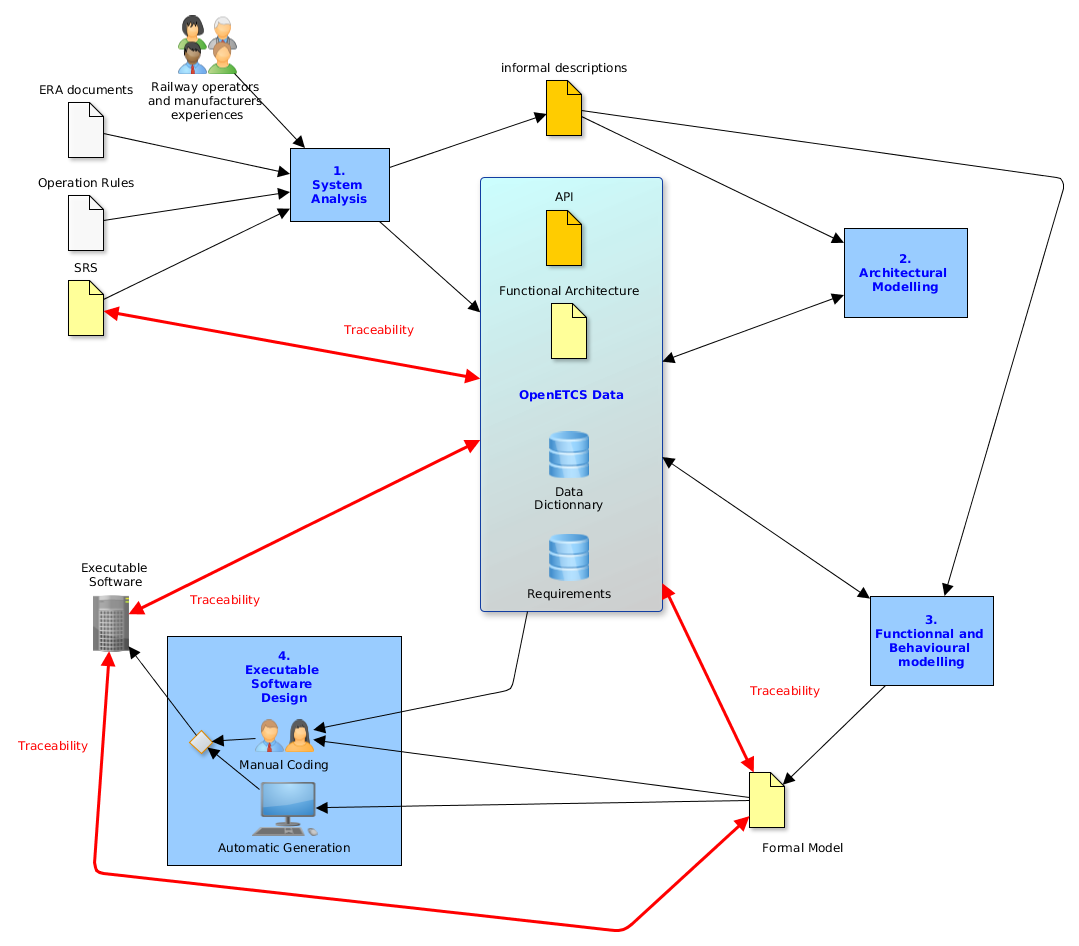
\includegraphics[width=\textwidth]{images/Step.png}
  \caption{Main steps of the design approach}
  \label{fig:Steps}
\end{figure}


\subsubsection{System analysis}

\paragraph{Aim}
The objectives of this step is to clarify the scope of the study and to provide a detailed description of the chosen solution to cover the requirements of the main input document of the project  [SRS-Subset 26 v3.3.0].

Thus the tasks of this step  are:
\begin{itemize}
\item to define the scope of the model (more or less the OBU kernel);
\item to provide an architecture for this model (functional and software);
\item to lift ambiguities;
\item to detect errors and inconsistencies.
\end{itemize}


\paragraph{Input artifacts}

The input documents and elements of this activity are also inputs of the project as it is its first activity.
\begin{itemize}
\item SRS Subset 26 v3.3.0 is the reference document and can be viewed as an user need document.
\item All the documents provided by ERA according to the directive [CCS TSI ] available \url{http://www.era.europa.eu/Core-Activities/ERTMS/Pages/Set-of-specifications-2.aspx}.
\item Experience of the railway operators partners
\item Experience of the railway manufacturers partners
\item National and Operation Rules of the operators
\end{itemize}

\paragraph{Output artifacts}

The output shall provide a clear view of the system to design and will be composed of:

\begin{itemize}
\item a set of informal descriptions (scope of the process, description of the functions, behaviour of the system, ...)
\item  an API to  describe the environment of the system to design, its interfaces and its dynamic implementation
\item a functional architecture which identifies the functions to design and the interaction between these functions and with the environment
\item a data dictionary with description of the input and output variables of the system and all the internal variables needed to  describe the system and the interactions between the functions
\item all the requirements, allocated to function or data description, in natural language. The requirements from the SRS can be possibly split and rewritten in order to restrict their scope to the functions or to match the objects of the data dictionary. New requirements can be defined to describe specification choices or to clarify the behaviour of a function (for example according to the experience from a partner). Traceability issue is mandatory and shall be taken into account early.

\end{itemize}

\paragraph{Means}

The first element needed is a way to manage and organize informal descriptions (including text, pictures, tables,...). 

Functional architecture can be easily defined with BDD and IBD diagrams (see \ref{section:sysml}).
Data dictionary  and requirement sets shall be tool supported in order to link their contents to the functional architecture and to  be reused during the modelling, verification, validation and safety activities.

As functional architecture, data dictionary and set of requirements shall be linked together, and shall be defined to be used during all the project. Thus section \ref{sec:datamodel} give some specification of the items to define and some naming conventions.

\subsubsection{Architectural modelling}


\paragraph{Aim}
The objectives of this step is to design the software organisation of the function to implement and to clarify the interaction with the hardware and the environment of the software.


\paragraph{Input artifacts}

The input documents and elements of this activity are:
\begin{itemize}
\item a set of informal descriptions (scope of the process, description of the functions, behaviour of the system, ...)
\item the API
\item the functional architecture 
\item the data dictionary 
\item the requirements, allocated to function or data description, in natural language. 
\end{itemize}

\paragraph{Output artifacts}

The output shall provide :

\begin{itemize}
\item the input API updated and completed
\item the input functional architecture updated and completed
\item the input data dictionary updated and completed
\item a set of new requirement which described the design choices made during this step
\item traceability  with system analysis output
\end{itemize}

\paragraph{Means}

The software architecture shall be derived from the functional architecture provided during system analysis step. By the way the existing SysMl model can be completed here to describe the software architecture, then derived to a SCADE model (for exemple by using Scade system), as SCADE is the method firstly proposed to  design the software.

\subsubsection{Functional and behavioural modelling}


\paragraph{Aim}
The objectives of this step is 


\paragraph{Input artifacts}

The input documents and elements of this activity are:
\begin{itemize}
\item a set of informal descriptions (scope of the process, description of the functions, behaviour of the system, ...)
\item the updated API
\item the updated functional architecture 
\item the updated data dictionary 
\item the updated set of requirements, allocated to function or data description, in natural language. 
\end{itemize}


\paragraph{Output artifacts}

The output shall provide:
\begin{itemize}
\item a formal model of on-board unit
\item the updated data dictionary 
\item the updated set of requirements, formalized or justified
\item traceability  with system analysis and architecture modelling output
\end{itemize}

\paragraph{Means}

One of the objectives of the project is to provide a formal model of the on-board unit functionalities. The task consist to give a formal model of the functions and the requirements.
First decision proposed to use the SCADE approach for this activity.
Thus the task  consist, from the SCADE architectural model, to complete the behaviour of the functions in each node of the model. 


\subsubsection{Executable software}


\paragraph{Aim}
The objectives of this step is to provide a C code which implements the applicative part of the On-board Unit as defined during the system analysis. Target of the executable code is not identify to  allow its reuse in different environment.
However, constraints specify in the API document shall be covered.


\paragraph{Input artifacts}

The input documents and elements of this activity are :
\begin{itemize}
\item Scade Model
\item Software Specification Document
\item API
\end{itemize}

\paragraph{Output artifacts}

The output shall provide an executive software:

\begin{itemize}
\item C code of the applicative part of the on-board unit
\item Supporting documentation: at least Software Deployement Manual and Release Notes

\end{itemize}

\paragraph{Means}

The C code can be generated from the Scade model for most of the parts. For interfaces components or for components which the code can be optimized c code shall be automatically written.

In both cases, the production of C code shall follow the constraints defined in EN50128 for SIL4 software design.



\subsection{Data Model}
\label{sec:datamodel}

This section describes all the data shared by the different activities during the project.
These data shall be managed in a common repository which shall be the reference for specification, modelling and VnV activities.

Thanks to the choice of Eclipse platform, use of technologies available on Eclipse and XML files are the best candidates to store these items.

In the following, we give the specification of these items and the links between them. The specification of this data-model is based on an Ecore model. However it can be implemented with any means or tools, depending the decision of the project partners.

3 groups of data are defined: \emph{Variable}, \emph{Function} and \emph{Requirement}; for each group, a set of \emph{attributes} are defined to specify the group. These attributes are specified by a name, a cardinality and a type which can be a well  know type  (as boolean, string, integer,...) or a type defined explicitly for this model.

All these items share common attributes described in the following section. The \emph{Features} are defined to organize the items in group.
Finally the links between the groups are specified in the last section.


\subsubsection{Common attributes}

All the items are \textit{named} and have mandatory common attributes:
\begin{description}
\item [name] defined as a string and unique for each item, naming convention are defined in \ref{sec:naming};
\item[safety] a boolean tag to qualified the information as safety or not ;
\item[definition] to describe in a clear way the items, at least by a textual description. Links to picture or table can be added.
\end{description}

Some \textit{issues} can be associated to  each items. These issues are characterized by:
\begin{description}
\item[description] a textual explanation;
\item[closed] a boolean tag to qualified the state of the issue;
\item[owner] the person in charge of the issue.
\end{description}

\begin{comment}
TODO: do we need more information on issue , as author, ... ?

Do we need to link to github issue tracker ?
\end{comment}

The figure \ref{fig:Common} gives the Ecore model of these elements.

\begin{figure}[ht]
  \centering
  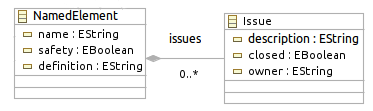
\includegraphics{DataModel/Common2.png}
  \caption{Common attributes for all items}
  \label{fig:Common}
\end{figure}


\subsubsection{Variables}
\label{sec:var}


First of all we have to define the types used to specify the variables.

In order of possible, we shall use simple and well defined, as boolean, string, integer,... (see the Iso standard for C language \url{http://www.open-std.org/jtc1/sc22/wg14/www/docs/n1124.pdf}). In the Ecore model these types appeared with the prefix "E".

Besides some new types can be added to define a complex or structured type or an enumeration.

These types are defined as \textit{VariableType} with the following attributes:
\begin{description}
\item[parentType] optional, in the case the type is a subtype of a  already defined type (for example "Distance" can be considered as subtype of "Integer");
\item[minimalValue] optional, in the case the type is a range of integer, the minimal value;
\item[maximalValue] optional, in the case the type is a range of integer, the maximal value;
\item[resolution] optional, in the case the type is a range of integer, resolution to take into account;
\end{description}

The figure \ref{fig:Type} gives the Ecore model of these elements.

\begin{figure}[ht]
  \centering
  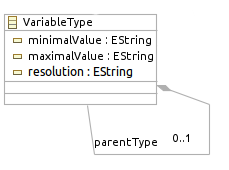
\includegraphics{DataModel/Type3.png}
  \caption{Type definition}
  \label{fig:Type}
\end{figure}

The \textit{Variable} is then defined with the following attributes:
\begin{description}
\item[type] the variableType associated, unique;
\item[definitionRequirements] at least one requirement to  define the variable;
\item[constant] a boolean tag to qualified constants;
\item[specialValue] optional, several special value can be defined;
\item[store] optional, a variable can be an element of a more complex or structured variable.
\end{description}

The figure \ref{fig:variable} gives the Ecore model of these elements.


\begin{figure}[ht]
  \centering
  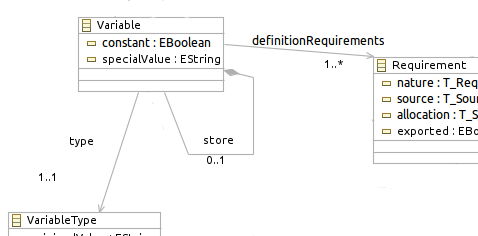
\includegraphics{DataModel/Variable3.png}
  \caption{Variable definition}
  \label{fig:variable}
\end{figure}



\subsubsection{Functions}

A \textit{Function} is defined with the following characteristics:
\begin{description}
\item[allocation] the subsystem  on which is allocated the function (i.e. Kernel, DMI, Odometry,..);
\item[requirement] at least one requirement to describe the function;
\item[input] optional, the input variables of the function;
\item[output] optional, the output variables of the function;
\item[internal] optional, the internal variables of the function;
\item[subFunction] optional, the sub-functions which allow to structure and  detailed the function.
\end{description}

The figure \ref{fig:function} gives the Ecore model of these elements.

\begin{figure}[ht]
  \centering
  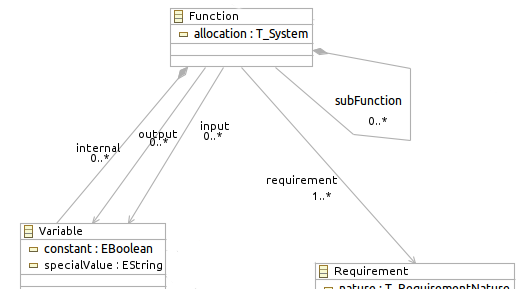
\includegraphics{DataModel/Function1.png}
  \caption{Function definition}
  \label{fig:function}
\end{figure}

\subsubsection{Requirements}
\label{sec:req}

A \textit{requirement} is defined by the following attributes:
\begin{description}
\item[nature] class of property defined by the requirement: Structural, functional, definition,...
\item[source] the document or the artifact where the requirement is defined for the first time (i.e. SRS, SystemAnalysis,...);
\item[allocation] the subsystem  on which is allocated the function (i.e. Kernel, DMI, Odometry,..);
\item[exported] a boolean tag to defined if the requirement shall be exported to another sub-system or function;
\item[subRequirement] optional, the sub-requirements in which the requirements is divided.
\end{description}

Thus the following enumerate sets shall be defined (their contents are not given in an exhaustive way here):
\begin{description}

\item[T\_SourceDocument] set of source document for defining a data, this can be an input document (SRS, a subset,...) or a document provided during the process (system analysis, model description,...) 
\item[T\_RequirementNature] what describe the requirement ? Structural, Functional or Definition
\item[T\_System] on what subsystem is allocated the data ? Kernel, DMI, BIU,...
\end{description}

The figure \ref{fig:requirement} gives the Ecore model of these elements.

\begin{figure}[ht]
  \centering
  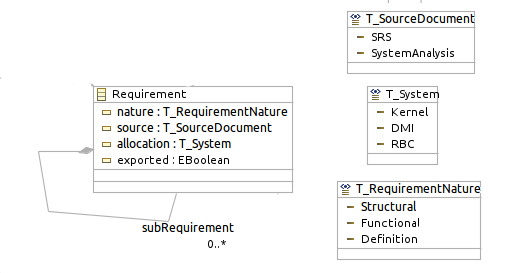
\includegraphics{DataModel/Requirement1.png}
  \caption{Requirement definition}
  \label{fig:requirement}
\end{figure}


\subsubsection{Feature}

A \textit{feature} is a mean to structure the analyse of the system, it is the starting element of an analysis, and contents informal information:
\begin{description}
\item[description] an informal and textual description of the functionality to analyse, which can contain some links to pictures or tables;
\item[subFunctions] the functions which are defined to describe the functionality.
\end{description}

The figure \ref{fig:feature} gives the Ecore model of these elements.

\begin{figure}[ht]
  \centering
  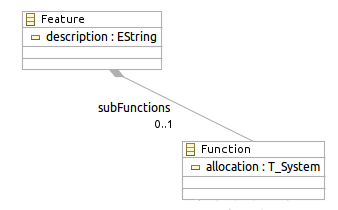
\includegraphics{DataModel/Feature1.png}
  \caption{Feature definition}
  \label{fig:feature}
\end{figure}

\subsubsection{Links}


The figure \ref{fig:links} gives the Ecore model of all the data model as describe above and can be read as an UML diagram.

\begin{figure}[ht]
  \centering
  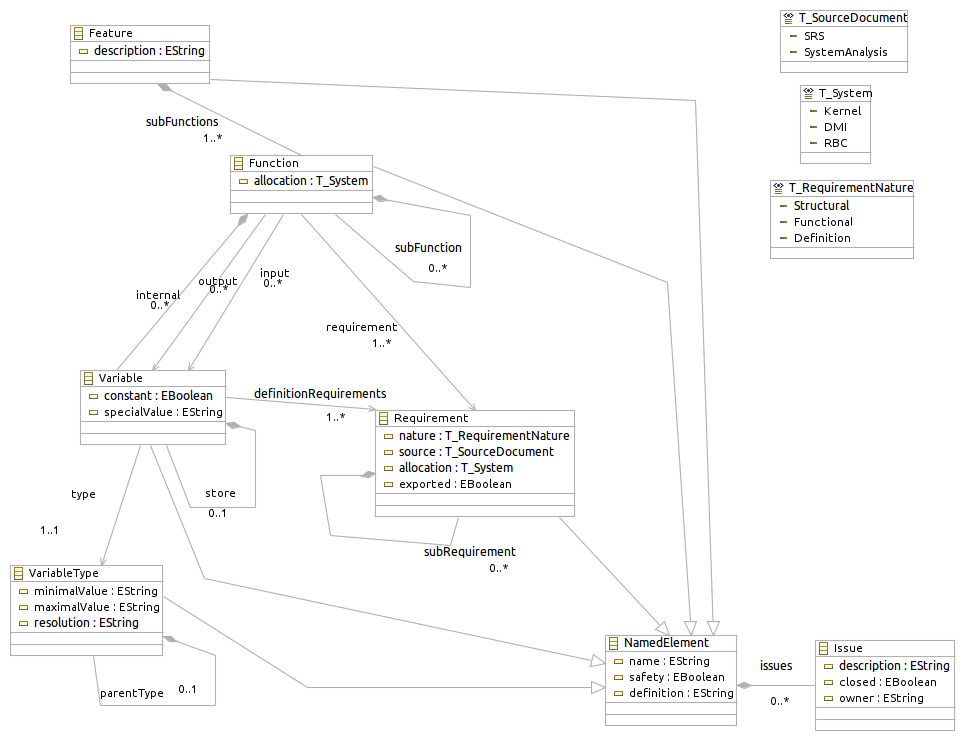
\includegraphics[width=\textwidth]{DataModel/datadictionary.png}
  \caption{General Ecore model of the data dictionnary}
  \label{fig:links}
\end{figure}

\subsection{Name convention}
\label{sec:naming}


All the items described in section \ref{sec:datamodel} shall be named in a unique way. 
This section gives some naming conventions to facilitate modelling and VnV.

In a general way, the name shall be clear, concise to facilitate the understanding of the models. UPPER case will be used for names issued form official documents as SRS, mixed of lower and UPPER case for others.

To avoid trouble during translation of models or code generation, we assume some languages can be not case sensitive: a same word can not be used twice with different cases. By the same way, classical keywords of programming language shall be avoid (for example for C language "if", "then", "void",...).




\subsubsection{VariableTypes naming convention}

The naming of the type should consist at least on an object.

The name shall be prefixed by "typ\_".

\subsubsection{Variable naming convention}

The naming of the variables should consist of at least a combination of a verb and an object using the passive form (for examples:   orderReceivedFromTrackside for a structure,     endOfMissionIsExecuted for a boolean)

For the internal variables, i.e. those defined during the design activities to describe the state of the system and the exchanges between functions, the name shall be prefixed by "int\_".

For the external variables, name shall be as close as possible to those already defined in the documentation.
Typically, the naming convention of SRS §7 and 8 shall be followed for the interface with trackside (see § 7.3.2.11):

\begin{itemize}
\item A\_ Acceleration
\item D\_ distance
\item G\_ Gradient
\item L\_ length
\item M\_ Miscellaneous
\item N\_ Number
\item NC\_ class number
\item NID\_ identity number
\item Q\_ Qualifier
\item T\_ time/date
\item V\_ Speed
\item X\_ Text
\end{itemize}

For the other external  variables, the name will be prefixed by the short name of the interface:

\begin{itemize}
\item DMI\_
\item ODO\_ for odometry
\item BTM\_
\item RIU\_
\item \dots
\end{itemize}

\subsubsection{Feature and Function naming convention}

Features and  functions are named using an active form consisting of at least a combination of a verb and an object (for example:   initiateTerminatingASession).

A short name, formed from first letters of each word, is defined for each feature to  facilitate the naming of sub-functions or requirements (for Example MORC for ManageOfRadioCommunication). 

\subsubsection{Requirement naming convention}

A requirement shall be identified in a unique way by is name and the  source document with it version.

The naming convention of requirement depends on the source document or activity as described in the following table:

\begin{tabular}{|p{2cm} | p{4cm} | p{8cm}|}
\hline 
Source & Name & Description \\
\hline 
Subset 26 v3.3.0 & SRS\_$number$\_$letter$ & where $number$ is the number of the section as it appears in the SRS, and $letter$, optional, is used in the case the requirement is divided in sub-requirements  (for example : 3.5.3.1, 3.5.3.4\_a) \\
\hline 
Subset X v Y & SubsetX\_Y\_$number$\_$letter$ &  where X is the number of the subset, Y its version, $number$ is the number of the section as it appears in the SRS, and $letter$, optional, is used in the case the requirement is divided in sub-requirements (for example : Subset\_34\_3.0.0\_ 2.2.2.1 \\
\hline 
System Analysis & SA\_$short$\_$number$ & where $short$ is the shortname of the feature or the allocated subsystem, $number$ is a unique number for this short name (for example SA\_MORC\_4 or SA\_DIM\_18) \\
\hline 
Software Modeling & SW\_$short$\_$number$ & where $short$ is the shortname of the feature or the allocated subsystem, $number$ is a unique number for this short name \\
\hline
\end{tabular}

\subsection{Use of the ETCS Language}
\label{sec:ETCSLanguage}

The ETCS Language, i. e. the definition of ETCS data types, packets and messages is specified in Subset 026, chapter 7 and 8. 

These definitions reflect the data formats at external interfaces, especially at the air gap between track and train. The data formats have been defined to save bits during their transmission between balises, loop, RBC and train. The various different bit lengths lead to field borders on bit boundaries in data structures and are very unhandy to be used in modelling and implementation languages. 

In addition, the ETCS language terminology talks about “variables” instead of “types”. For clarification: all “variable”, “packet” and “message” types are in fact data type definitions and should not be misunderstood as global variables. 
To unburden the OBU software modelling and implementation from the inconvenience of arbitrary bit lengths and bit boundaries, the following provisions should be made.

\subsubsection{Transformations between native ETCS language and OBU internal data types}

The ETCS language data types as specified in  Subset 026, chapter 7 and 8, require an OBU software internal equivalent supported by the openETCS modeling and implementation languages.  

Native ETCS language data types must be converted into OBU internal data types at the external interfaces of the OBU software.
This enables the internal OBU functions to deal with internal data types only. 

\subsubsection{Mapping of basic data types: Native ETCS language - OBU internal data types}

The transformations between ETCS data types and the corresponding OBU internal data types are

		\begin{tabular}{|p{7cm} | p{7cm} |}
			\hline 
				Native ETCS language types & OBU internal data types \\
			\hline 
			integer 2 – 31 bit & integer32  \\
			\hline 
			enumeration & enumeration \\
			\hline 
			integer 1 bit & boolean (if character is boolean) \\
			\hline 
			integer 1 bit & enumeration (if character is enum) \\
			\hline 
			physical dimensions w. int resolution & integer or fixed point \\
			\hline 
			structures & structures with fields on at least byte boundaries \\
			\hline 
			dynamic iterations of structures & Iterations unrolled and transformed into static arrays of structures of constant maximum size (constant defined in a central place, minimum = 0) \\
			\hline 
			
		\end{tabular}

\subsubsection{Mapping of type names}

To avoid confusion by different names for internal and external data types and preserve the relationship between both, types defined in the ETCS language shall preserve their names when transformed into their corresponding OBU internal data type. The distinction between both shall be made via different name spaces and prefixes only. 

\subsubsection{Use of ETCS language type definitions whenever possible}

In principle, data type used internally within the ETCS OBU software can be defined freely. 
On the other hand, the distributed development in the openETCS team could be improved by common understanding and agreement to artefacts defined by the ETCS language.

Therefore, self defined data types shall be based upon ETCS language elements (transformed to the internal equivalent) whenever possible.
Type definitions in parallel to existing ETCS language terms shall be avoided. 

\subsubsection{Uniform scaled (physical) dimensions}

Several elements of the ETCS language use combinations of scaling factors (example: Q\_SCALE) and values (example: D\_LINK) to quantify (physical) dimensions. 
Self-defined OBU internal types shall be based upon a unique scaling factor instead (example: all lengths and distances in cm).

\subsubsection{Replacing dynamic data structures with static type definitions}

Several structured types of the ETCS language use iterations of substructure loops of arbitrary lengths; an actual iterator value then indicates the actual length of the loop. 
Since such dynamic allocations are not suited for dependable and safety-related software, the dynamic structures shall be replaced by static structure arrays of a constant maximum length. 
“dataValid”-Flags (see next sectionh) then shall designate array elements filled with data.

Default values should be assigned to “empty” variables additionally.


\subsection{Basic Concepts}
\label{sec:BasicConcepts}

\subsubsection{"`dataValid"'-Flags and "`eventValid"'-Strobes}

Since resource allocations like memory space for variables must not be performed dynamically, all resources must be allocated statically and variables like structures and arrays must be of fixed size. This requires a method to differentiate the array elements or structures filled with valuable data from "`empty"' ones. This shall be achieved by adding a boolean “dataValid” flag to the structures and array elements. 
Data flows with event character (example: a just received balise datagram) shall in the same way make use of such “valid” strobes within the data flow type definitions: a “eventValid” strobe set to true then designates the presence of an event, set to false designates the absence of an event. 

Default values should be assigned to “empty” variables additionally.

\subsubsection{Time Stamps}

All data received via an external or internal interface (like sensors, balise antennas, ...) shall be marked with the actual system time at the earliest moment of reception.

This allows to eliminate the impact of system internal propagation delays and can be used consistency checks or for diagnosis purposes, if neccessary.

\subsubsection{Execution on a Synchronously Clocked Platform}

The openETCS software has to be modeled and implemented to be executed on a synchronously clocked platform or runtime system with the following characteristics.

A clock cycle is divided into exactly 3 phases: 

\begin{enumerate}
	\item Sample and hold of all inputs (input phase)
	\item Calculate all outputs (execution phase)
	\item Emit all outputs (output phase)
\end{enumerate}

The execution order of subfunctions results from the input-output relationships between the subfunctions. There are no racing conditions between subfunctions.

Whithin one clock cycle, the system time (as all other inputs to the OBU software) is kept unchanged for the OBU software. The processing time for all 3 phases is thought to be 0 (practically, it will be > 0, but this is irrelevant as long as the processing time does not exceed the clock period).

